% Figure from MATH 591 notes, section 67. After the board (Lecture 24): the Euler field.
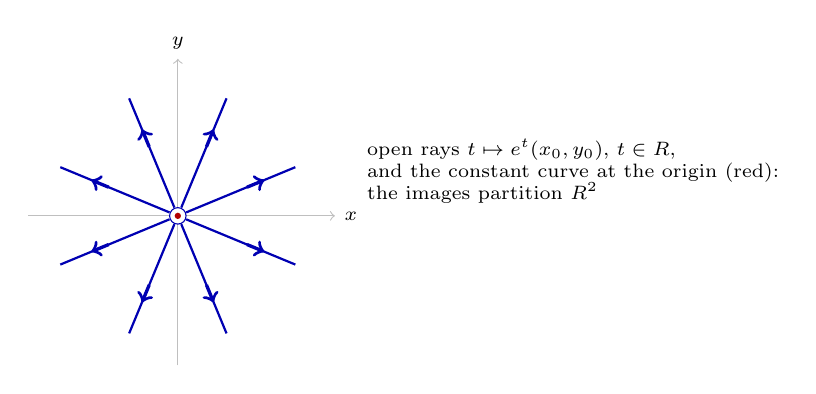
\begin{tikzpicture}[scale=0.95]
\draw[->, gray!50] (-2,0) -- (2.1,0) node[right, font=\scriptsize, text=black] {$x$};
\draw[->, gray!50] (0,-2) -- (0,2.1) node[above, font=\scriptsize, text=black] {$y$};
\draw[blue!70!black, thick] (0.111,0.046) -- (1.571,0.651);
\draw[->, blue!70!black, very thick] (0.924,0.383) -- (1.155,0.478);
\draw[blue!70!black, thick] (0.046,0.111) -- (0.651,1.571);
\draw[->, blue!70!black, very thick] (0.383,0.924) -- (0.478,1.155);
\draw[blue!70!black, thick] (-0.046,0.111) -- (-0.651,1.571);
\draw[->, blue!70!black, very thick] (-0.383,0.924) -- (-0.478,1.155);
\draw[blue!70!black, thick] (-0.111,0.046) -- (-1.571,0.651);
\draw[->, blue!70!black, very thick] (-0.924,0.383) -- (-1.155,0.478);
\draw[blue!70!black, thick] (-0.111,-0.046) -- (-1.571,-0.651);
\draw[->, blue!70!black, very thick] (-0.924,-0.383) -- (-1.155,-0.478);
\draw[blue!70!black, thick] (-0.046,-0.111) -- (-0.651,-1.571);
\draw[->, blue!70!black, very thick] (-0.383,-0.924) -- (-0.478,-1.155);
\draw[blue!70!black, thick] (0.046,-0.111) -- (0.651,-1.571);
\draw[->, blue!70!black, very thick] (0.383,-0.924) -- (0.478,-1.155);
\draw[blue!70!black, thick] (0.111,-0.046) -- (1.571,-0.651);
\draw[->, blue!70!black, very thick] (0.924,-0.383) -- (1.155,-0.478);
\draw[blue!70!black, fill=white] (0,0) circle (0.11); \fill[red!70!black] (0,0) circle (1.2pt);
\node[font=\scriptsize, anchor=west, align=left] at (2.4,0.6) {open rays $t \mapsto e^t(x_0, y_0)$, $t \in \mathbb{R}$,\\ and the constant curve at the origin (red):\\ the images partition $\mathbb{R}^2$};
\end{tikzpicture}
